\chapter{State of the Art}\label{chapter:state-of-the-art}
This chapter presents an overview of state of the art approaches to object recognition, while focusing on two families of artificial neural network (ANN) architectures, which are motivated quite differently. Object recognition techniques based on \emph{convolutional neural networks} (CNNs) currently dominate the field, achieving state of the art performance by a large margin over classical methods on many datasets \cite{Diba2017WeaklySC,7506134}. Even though CNNs were originally inspired by findings from neuroscience, by now they have diverged quite a bit from the computational models used to study the brain. The neurorobotics approach to cognitive systems, based on \emph{spiking neural networks} (SNNs) on the other hand, attempts to mimic the animal brain by more closely modelling the physical properties and behavior of neurons and therefore results in biologically more plausible models \cite{Schofield20180027}. Generally speaking, CNNs may be regarded as a more engineering-based approach (or top-down), while SNNs are motivated by results from neuroscience and biology (bottom-up approach).
\begin{figure}
    \centering
\begin{tikzpicture}
  \node[anchor=south west,inner sep=0] at (0,0) {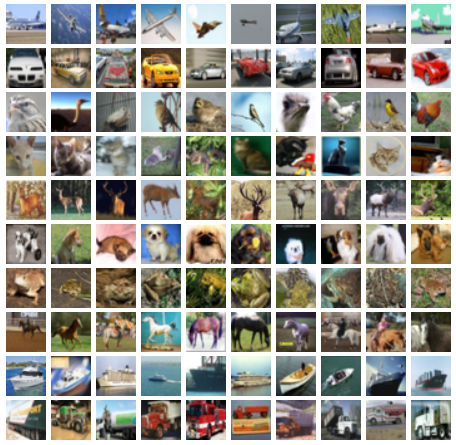
\includegraphics{figures/cifar10.png}};
  \node[anchor=west] at (-2.5,8.9) {Airplane};
  \node[anchor=west] at (-2.5,7.95) {Automobile};
  \node[anchor=west] at (-2.5,7.05) {Bird};
  \node[anchor=west] at (-2.5,6.1) {Cat};
  \node[anchor=west] at (-2.5,5.2) {Deer};
  \node[anchor=west] at (-2.5,4.25) {Dog};
  \node[anchor=west] at (-2.5,3.35) {Frog};
  \node[anchor=west] at (-2.5,2.45) {Horse};
  \node[anchor=west] at (-2.5,1.5) {Ship};
  \node[anchor=west] at (-2.5,.55) {Truck};
\end{tikzpicture}
\caption[CIFAR-10 classes and sample images]{Sample images from the CIFAR-10 \cite{cifar10} dataset and their corresponding classes. CIFAR-10 consists of 6000 images at 32 by 32 pixels for each of the 10 classes. Datasets such as this are often used as a benchmark to evaluate the performance of novel ANN architectures for image recognition. This is done by using a subset of the dataset (often referred to as the training set) to train the neural network. The remainder of the images (accordingly called the test set), which the network has not seen before, are used to evaluate the classification accuracy.}\label{fig:cifar10}
\end{figure}\noindent
\section{Artificial Neural Networks for Object Recognition}
Recent years have seen a surge of interest in artificial neural networks and deep learning methods, especially in the field of computer vision. While the theory for training such networks has been around for many years, their recent success is mainly due to the availability of large labelled data sets (so called big data) and the proliferation of highly parallel computing powered by GPUs. One of the specific tasks, deep learning based methods excel at, is object recognition\footnote{In machine learning, tasks such as object recognition are referred to as classification problems. The resulting classifiers are part of a broader class of methods called \emph{supervised learning}. In supervised learning, the desired output (i.e. the label) has to be provided for all the samples used for training the classifier.}: the identification of objects in images or videos (cf. figure \ref{fig:cifar10}). The significantly better performance of deep neural networks over traditional machine learning methods can be explained by: (i) their hierarchical topology of parameterized non-linear processing units is a fundamentally better probabilistic model and prior for real world data as captured in images leading to better generalization and (ii) they autonomously find good features to extract based on the training data. Interest is further fueled by the myriad potential applications of robust object recognition systems: from automated driving and image-based diagnosis in medicine to robot vision and many more. As deep learning is currently the best candidate for such a system, it is well worth exploring.
\section{Convolutional Neural Networks}\label{section:cnn}
CNN architectures are generally distinguished by their use of specific types of neuron-layers, namely, convolutional, pooling and fully connected layers. While wildly different network topologies may be found in literature, characterized by their use of skip connections, number of layers, number of paths etc., CNNs can always be reduced to these three basic layer types.
\subsubsection{Fully Connected Layer}
Each neuron in a fully connected layer is connected to all the activations in the previous layer. The activation of a single neuron (cf. figure \ref{fig:neuron}) is calculated by applying a nonlinearity to the weighted sum of its inputs and a bias.
\begin{align}
    h = g\qty(\sum_i w_i x_i +b)
    \label{eq:neuron}
\end{align}
\begin{figure}
    \centering
\begin{tikzpicture}
  \node[anchor=south west,inner sep=0] at (0,0) {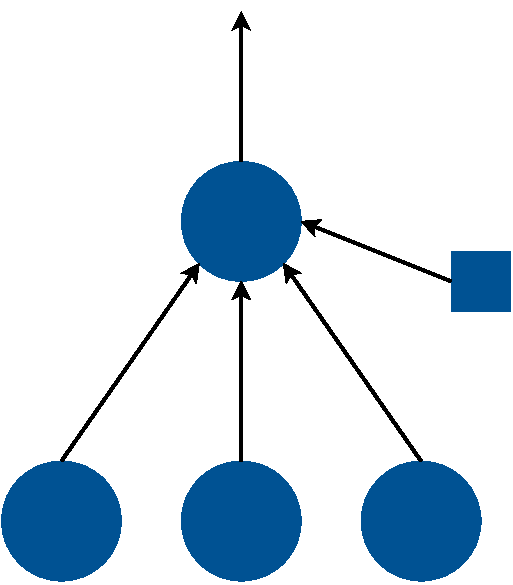
\includegraphics[scale=.5]{figures/Neuron.pdf}};
  \node[anchor=west] at (.2,1.8) {$w_1$};
  \node[anchor=west] at (1.3,1.8) {$w_2$};
  \node[anchor=west] at (2.3,1.8) {$w_3$};
  \node[anchor=west] at (4.3,2.6) {$b$};
  \node[anchor=west] at (.2,-.5) {$x_1$};
  \node[anchor=west] at (1.75,-.5) {$x_2$};
  \node[anchor=west] at (3.3,-.5) {$x_3$};
  \node[anchor=west] at (1.3,4.2) {$h$};
\end{tikzpicture}
\caption[Illustration of an artificial neuron with three input connections]{Illustration of an artificial neuron with three input connections. Artificial neurons constitute the basic non-linear computational units of neural networks. The neuron receives the activations of three lower level neurons weighted by the learnable $w_i$ as well as a learnable bias $b$. After applying the nonlinearity (also known as activation function), the neuron outputs its activation $h$ as in equation  \ref{eq:neuron}}\label{fig:neuron}
\end{figure}\noindent
With the nonlinear function $g$, the learnable weights $w_i$, the input activations $x_i$ and the learnable bias $b$. In the case of a fully connected layer, the activations can be computed using matrix multiplication. In tensor notation this may be written as:
\begin{align}
    \vb{h_l} = g_l\qty(\vb{W^T_l\vb{h_{l-1}}}+\vb{b_l}).
\end{align}
With $N_l$ denoting the number of neurons in layer $l$, $\vb{W_l}$ is an $N_{l-1}\cp N_l$ dimensional weight matrix, $b_l$ an $N_l$ dimensional vector and $g_l$ the $N_l$ dimensional vectorized activation function of layer $l$.
\begin{align}
    g_l(\vb{x}) = \qty(g_l(x_1),...,g_l(x_{N_l}))^T
\end{align}
The computational power of neural networks is shown by the universal approximation theorem. The theorem states that networks with a single hidden layer (cf. figure \ref{fig:fully-connected}) containing a finite number of neurons can approximate arbitrary continuous functions on compact subsets of $\mathbb{R}^n$ \cite{univ-approx-1,univ-approx-2}.
\begin{figure}
    \centering
\begin{tikzpicture}
  \node[anchor=south west,inner sep=0] at (0,0) {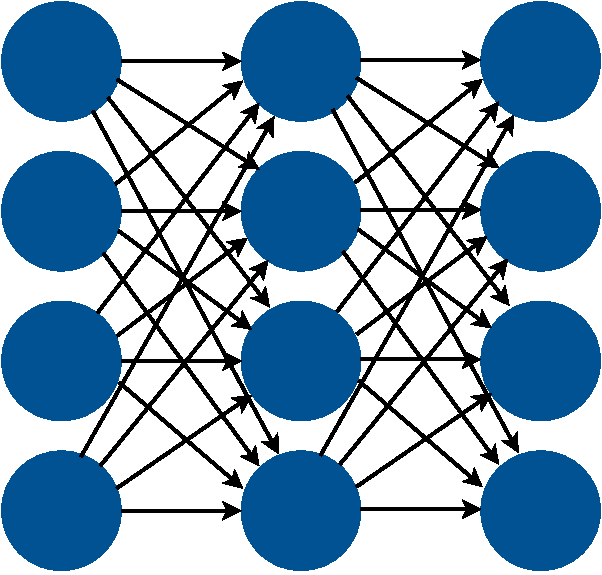
\includegraphics[scale=.5]{figures/FullyConnected.pdf}};
  \node[anchor=west] at (.2,-.5) {$h_0$};
  \node[anchor=west] at (2.3,-.5) {$h_1$};
  \node[anchor=west] at (4.3,-.5) {$h_2$};
\end{tikzpicture}
\caption[Illustration of fully connected layers]{Illustration of a fully connected neural network as a directed graph with input layer $h_0$ and output layer $h_2$. Layers between the input and output layer are usually referred to as \emph{hidden} layers. Note that the biases are not explicitly shown.}\label{fig:fully-connected}
\end{figure}\noindent
\subsubsection{Convolutional Layer}
In a convolutional layer, the activities of the input layer are convolved with a number of trainable kernels so as to create the same number of feature maps. In computer vision it is common to view the layer's neurons as two-dimensional grids of neurons arranged in channels (cf. figure \ref{fig:2dconvolution}). These grids correspond to pixels and color channels in the case of the input layer or activities (feature maps) resulting from convolution with different kernels in the case of intermediate convolutional layers. For a feature kernel $F_{m,n}^l$ of size $M_l\cp M_l$ and an input layer $l-1$ with $N_{l-1}\cp N_{l-1}$ neurons, the corresponding feature map activities of layer $l$ are computed as
\begin{align}
    h^l_{m,n} = g_l\qty(\sum_{m'}^{M_l}\sum_{n'}^{M_l}F_{m',n'}^l h_{m+m',n+n'}^l+b_l).
    \label{eq:2dconv}
\end{align}
This is the same as a two-dimensional discrete cross correlation.
\begin{align}
    (f \star g)[n]\ \stackrel{\mathrm{def}}{=} \sum_{m=-\infty}^{\infty} f^*[m]\ g[m+n]
\end{align}
Where $f^*$ is the complex conjugate of the discrete function $f$. Strictly speaking, the use of the term \emph{convolution} in neural network literature is therefore a misnomer, as either the filter or the image (or feature map) would have to be flipped before the operation. However, as the weights of the kernel are actually learned by the network, the result will be the same. 

For a 2D single channel input layer of size $N_0\cp N_0$, the number of trainable parameters for a convolutional layer with a single $M\cp M$ filter is $M^2 + 1$ for the kernel weights and bias respectively, compared to $N_0^2N_1^2+N_1^2$ for a fully connected layer of size $N_1\cp N_1$. The sparsity in learnable parameters in convolutional layers compared to fully connected layers (cf. figure \ref{fig:convolutional}) is often referred to as \emph{weight sharing} (an entire channel \emph{shares} the weights of a single kernel).

In the case of multiple input channels, the kernels actually extend through the whole depth of the input layer's volume. Equation \ref{eq:2dconv} can be extended to accommodate multiple input channels and feature kernels. The activities of feature map $k$ in layer $l$ are then computed as
\begin{align}
    h^l_{k,m,n} = g_l\qty(\sum_{k'}^{K_{l-1}}\sum_{m'}^{M_l}\sum_{n'}^{M_l}F_{k,k',m',n'}^l h_{k',m+m',n+n'}^l+b_{l,k}).
    \label{eq:conv-multilayer}
\end{align}
With $K_l$ the number of channels in layer $l$. Most deep learning frameworks offer additional hyperparameters for convolutional layers, like stride and zero padding. Zero padding adds additional rows and columns of zero-activities around the input layer channels, effectively allowing the output feature maps to have the same size (i.e. height and width, depth is determined by the number of kernels) as the unpadded input layer. Stride on the other hand defines the integer value by which the kernels are moved during convolution. This can be used to keep the receptive fields from overlapping too much. Equation \ref{eq:conv-multilayer} is easily extended to take the stride $S_l$ of layer $l$ into consideration.
\begin{align}
    h^l_{k,m,n} = g_l\qty(\sum_{k'}^{K_{l-1}}\sum_{m'}^{M_l}\sum_{n'}^{M_l}F_{k,k',m',n'}^l h_{k',S_l m+m',S_l n+n'}^l+b_{l,k})
\end{align}
The spatial dimension of this feature map can be computed as a function of the input layer size $N_{l-1}\cp N_{l-1}$ and the amount of zero padding $P_l$.
\begin{align}
    N_l = \frac{N_{l-1}-M_l+2P_l}{S_l}+1
\end{align}
\begin{figure}
    \centering
\begin{tikzpicture}
  \node[anchor=south west,inner sep=0] at (0,0) {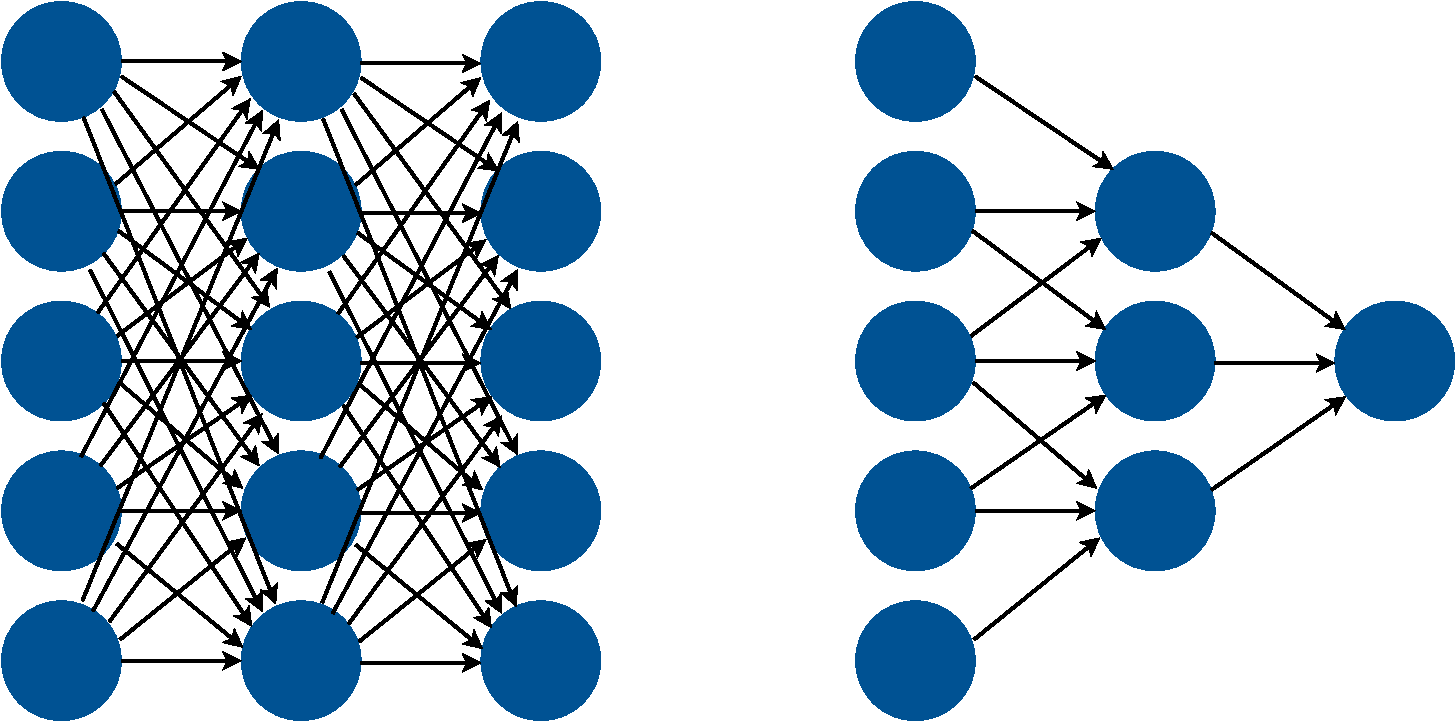
\includegraphics[scale=.5]{figures/Convolutional.pdf}};
  \node[anchor=west] at (.2,-.5) {$h_0$};
  \node[anchor=west] at (2.3,-.5) {$h_1$};
  \node[anchor=west] at (4.3,-.5) {$h_2$};
  \node[anchor=west] at (7.5,-.5) {$h'_0$};
  \node[anchor=west] at (9.6,-.5) {$h'_1$};
  \node[anchor=west] at (11.6,-.5) {$h'_2$};
\end{tikzpicture}
\caption[Illustration of convolutional layers]{Illustration of fully connected layers compared to convolutional layers, making apparent the sparsity of the latter relative to the former. The convolutional layers $h'_1$ and $h'_2$ perform a 1D convolution with a filter of size $3$. Note that due to weight sharing the number of weight parameters between $h'_0$ and $h'_1$ is actually only $3$. Also note that convolution reduces the number of neurons (or pixel resolution in the case of an image). For an input layer with $N$ neurons and a filter kernel of size $M$ the number of neurons in the convolutional layer computes as $N-M+1$. }\label{fig:convolutional}
\end{figure}\noindent
\begin{figure}
    \centering
\begin{tikzpicture}
  \node[anchor=south west,inner sep=0] at (0,0) {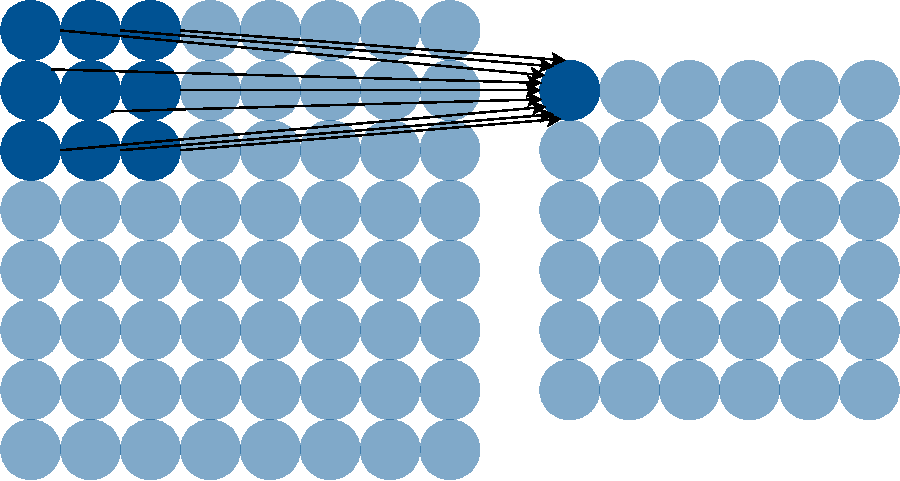
\includegraphics[scale=.5]{figures/2DConvolution.pdf}};
  \node[anchor=west] at (.4,4.5) {$M_l$};
  \node[anchor=west] at (-1,3.3) {$M_l$};
  \node[anchor=west] at (1.8,-.5) {$h_0$};
  \node[anchor=west] at (5.8,-.5) {$h_1$};
\end{tikzpicture}
\caption[Illustration of receptive field in 2D convolutional layer]{Illustration of a 2D convolution with a kernel of size $M_l\cp M_l$. As the resulting feature map $h_1$ has a lower resolution than $h_0$, applying a convolutional layer is sometimes also referred to as downsampling. For an input layer with $N\cp N$ neurons, the feature map's size is computed as $(N-M_l+1)\cp (N-M_l+1)$. The area comprised of the input neurons that are used to calculate the activity of a feature map neuron (highlighted neurons in layer $h_0$) are known as that neuron's \emph{receptive field}.}\label{fig:2dconvolution}
\end{figure}\noindent
\subsubsection{Pooling Layer}
Pooling is a form of sub- or downsampling using a sliding window similar to convolution. Most often the stride is set equal to the window size - that way the windows don't overlap. An operator is applied to each window, which selects a single neuron. Common operators are maximum, average or $L_2$-Norm. The pooling is applied to each channel and leads to a reduction in the spatial dimensions. This reduction corresponds to a loss of information or reduction in degrees of freedom and therefore reduces the amount of computation required as well as the possibility of overfitting. The choice of pooling operator has a profound effect on the generalization and speed of convergence of CNNs and recently maximum pooling has proven to be the most successful method \cite{pooling1,pooling2}.
\begin{figure}
    \centering
\begin{tikzpicture}
  \node[anchor=south west,inner sep=0] at (0,0) {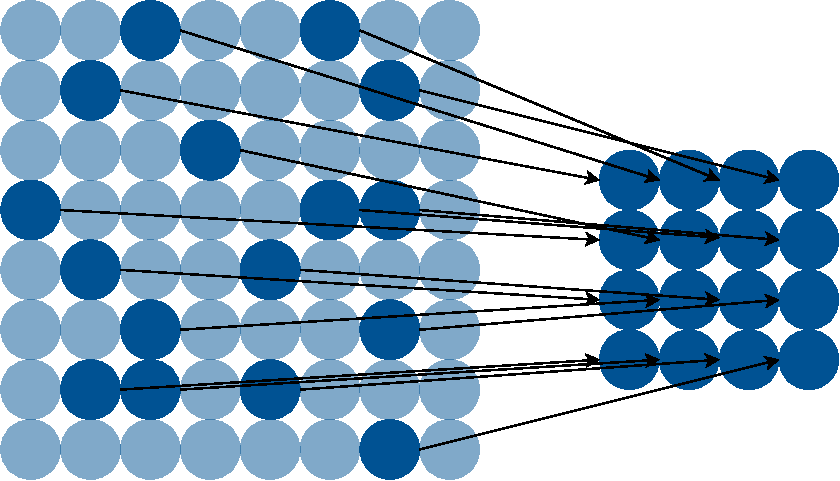
\includegraphics[scale=.5]{figures/Pooling.pdf}};
  \node[anchor=west] at (1.8,-.5) {$h_0$};
  \node[anchor=west] at (5.8,-.5) {$h_1$};
  \draw [decorate,decoration={brace,amplitude=5pt},xshift=-4pt,yshift=0pt]
(-0.1,3.1) -- (-0.1,4.05) node [black,midway,xshift=-0.6cm] {$M_l$};
  \draw [decorate,decoration={brace,amplitude=5pt},xshift=-4pt,yshift=0pt]
(.15,4.3) -- (1.2,4.3) node [anchor=south,midway,yshift=1] 
{$M_l$};
\end{tikzpicture}
\caption[Illustration of a pooling layer]{Illustration of a pooling layer. The pooling uses a $2\cp 2$ window with stride 2 to segment the input layer into non-overlapping tiles. An operator (e.g. maximum) is applied to each $2\cp 2$ segment to select a single neuron (the highlighted neurons in layer $h_0$). The activities of the selected neurons are aranged in a new layer $h_1$ of size $\frac{N_{l-1}}{M_l}\cp \frac{N_{l-1}}{M_l}$ with $M_{l}\cp M_{l}$ and $N_{l-1}\cp N_{l-1}$ the size of the window and the input layer respectively.}\label{fig:pooling}
\end{figure}\noindent
\subsubsection{CNN Architecture}
The key idea behind the combination of these three types of layers is that essential visual features such as edges and corners within a convolutional layer's receptive field are combined to form higher level features such as shapes by subsequent convolutional layers. In between these convolutions, pooling operations select the most salient features and reduce the computational size of the network. The convolutional kernels are effectively trainable feature detectors and due to weight sharing and pooling naturally incorporate a measure of translational invariance. This hierarchical organization of receptive fields is similar in structure to the mammalian visual cortex \cite{cat-brain} and sometimes CNNs are seen to be directly derived from it \cite{Fukushima1980,lecun2015deep}. More often than not however, the use of convolutional layers with weight sharing is motivated as a means to achieve translational equivariance and faster computation compared to fully connected layers \cite{Goodfellow-et-al-2016,7298668,7298594}. Finally, fully connected layers are placed on top of the network in order to perform high level inference (cf. figure \ref{fig:cnn-arch}). A CNN's architecture is therefore largely defined by its topology: the number and types of layers as well their neurons and the connections between them. The number of stacked layers is referred to as the network's depth. Current networks often employ multiple paths and skip connections (i.e. a layer's output not only flows to its direct descendent, but skips several layers) allowing for topologies several hundred layers deep, hence \emph{deep learning} \cite{huang2017densely,szegedy2017inception,xie2017aggregated,wang2015towards}.
\begin{figure}
    \centering
\def\svgwidth{\textwidth}
\import{figures/}{AlexNet.pdf_tex}
\caption[Illustration of a typical CNN architecture]{Illustration of a typical CNN architecture for object recognition. Note that the feature maps of the first convolutional layer extracted elementary features like edges. The last layer's neurons correspond to the trained classes, while the output neuron with the highest probability is picked as the network's prediction during inference (highlighted in red).}\label{fig:cnn-arch}
\end{figure}\noindent
\subsubsection{Training}
For object recognition, the output of the final layers are the class probabilities. This is achieved by applying a normalizing activation function to the the output of the last layer, such as the \emph{softmax} function. In case of the softmax function, the network's output $y_k\qty(\vb{x})$ for the class $k$ given input sample $\vb{x}$ thus becomes
\begin{align}
    y_k\qty(\vb{x}) = \frac{\exp(a_k)}{\sum_{k'=1}^K \exp(a_{k'})}.
\end{align}
With $\vb{a}=(a_1,...,a_K)^T$ the linear activities of the last layer's neurons (in machine learning literature often referred to as \emph{logits}) and $K$ the number of classes. Using one-hot coding for the target class
\begin{align}
    \vb{t} = (t_1,...,t_k,..,t_K)^T = (0,...,1,...,0)^T,
\end{align}
the probabilistic model can be defined as a function of the neural network.
\begin{align}
    P\qty(\vb{t}\mid \vb{x},\vb*{\theta}) = \prod_{k=1}^K y_k\qty(\vb{x})^{t_k}
\end{align}
With $\vb*{\theta}=(\vb{W}, \vb{b})$ the set of the network's trainable parameters. The model's likelihood is then given by
\begin{align}
    P\qty(\vb{T}\mid \vb{X}, \vb*{\theta}) &= \prod_n P(\vb{t_n}\mid\vb{x_n},\vb*{\theta}).
\end{align}
Where the index $n$ denotes $n$th training sample and target class (also known as label). The negative logarithm of the likelihood, called the negative \emph{log-likelihod} defines the classifier's error function $E_{\mathrm{ML}}$.
\begin{align}
    E_{\mathrm{ML}}\qty(\vb*{\theta}) &= -\log(P\qty(\vb{T}\mid \vb{X}, \vb*{\theta})) = -\sum_n \log P(\vb{t_n}\mid\vb{x_n},\vb*{\theta}) \\ &= -\sum_n \sum_{k=1}^K t_{n,k}\log(y_{k}\qty(\vb{x_n})) \label{eq:cross-entropy}
\end{align}
The error function resulting from the softmax activation function specifically is referred to as the \emph{cross entropy} (equation \ref{eq:cross-entropy}). Now the network's parameters may be trained by minimizing its classification error w.r.t. $\vb*{\theta}$. As the logarithm is a convex function and the error function is the \emph{negative} log-likelihood, this is equivalent to a maximum likelihood estimate. The gradient of the error function can be computed using the derivative chain rule (cf. figure \ref{fig:computegraph}), this method is known as \emph{backpropagation} and forms the computational backbone of CNN architectures.
\begin{align}
    \pdv{E_{\mathrm{ML}}\qty(\vb*{\theta})}{\vb*{\theta_{l-1}}} &= \pdv{E_{\mathrm{ML}}\qty(\vb*{\theta})}{h_{l-1}} \pdv{h_{l-1}}{\vb*{\theta_{l-1}}} = \pdv{E_{\mathrm{ML}}\qty(\vb*{\theta})}{h_l}\pdv{h_l}{h_{l-1}} \pdv{h_{l-1}}{\vb*{\theta_{l-1}}}
\end{align}
\begin{figure}
    \centering
\def\svgwidth{\textwidth}
\import{figures/}{computegraph.pdf_tex}
\caption[Computational graph for error propagation]{Computational graph for error propagation within a neural network. a) shows the dependency of the layers on both the lower layer's output as well as the parameters $\vb*{\theta_l}$ during inference (also known as forward pass). In b) the computational nodes for the error gradient as needed for error backpropagation were added (known as the backward pass).}\label{fig:computegraph}
\end{figure}\noindent
The gradient calculated based on the training samples is then used to update the network's parameter.
\begin{align}
    \vb*{\theta}^{(s+1)} &= \vb*{\theta}^{(s)}-\eta \grad{E_{\mathrm{ML}}\qty(\vb*{\theta}^{(s)})}
\end{align}
Where $s$ counts the number of training epochs (a run through all the samples) and $\eta$ is a hyperparameter known as the \emph{learning rate}, that effectively describes the size of the step taken in direction of the gradient (cf. figure \ref{fig:errorsurf}). In practise, the gradient is often calculated as an average based on a subset of randomly selected training samples.
\begin{align}
    \vb*{\theta}^{(s+1)} &= \vb*{\theta}^{(s)}-\eta\frac{1}{M} \sum_{n=1}^M\grad{E_n\qty(\vb*{\theta}^{(s)})}
\end{align}
The $\frac{N}{M}$ sets of training samples are called (mini-) \emph{batches} and are trained sequently until all samples have been seen, completing an epoch. Training algorithms based on this optimization scheme are known as \emph{stochastic gradient descent} (SGD). It is at this point that vectorization libraries are used to leverage the power of modern GPUs by processing an entire mini batch in parallel.
\begin{figure}
    \centering
\def\svgwidth{.5\textwidth}
\import{figures/}{errorsurface.pdf_tex}
\caption[Illustration of a neural network's error function]{Illustration of the surface of a neural network's error function in parameter space. The function is non-convex and contains a local minimum. Note that the resulting minimum depends on both the learning rate and the initialization of the parameters. In this case, following the negative gradient (illustrated as a red arrow) using small steps will converge on a non-optimal local minimum.}
\label{fig:errorsurf}
\end{figure}\noindent

State of the art CNN architectures expand upon the building blocks introduced in this chapter in various ways depending on the application. Often it is necessary to regularize the network's weights in order to prevent overfitting. This can be achieved by adding penalties for large weights to the loss function (known as weight decay) or randomly setting some weights to zero during training (so-called dropout) \cite{srivastava2014dropout,pmlr-v28-wan13,krogh1992simple,treadgold1998simulated}. This can be complemented with adaptive learning schemes\footnote{Adaptive extensions to SGD try to adjust learning hyperparameters like the learning rate based on performance on training data. It is for example quite common to decrease the learning rate after each training epoch that didn't increase accuracy or use such a scheme with independent learning rates for each weight.} in order to reliably train neural networks \cite{zeiler2012adadelta,duchi2011adaptive,kingma2014adam,polyak1992acceleration,graves2013generating,sutskever2013importance,loshchilov2016sgdr}. To make the process of training a neural network even more robust and prevent the gradients from becoming either too large or too small, it has proven useful to normalize a layer's input. In addition to stabilizing training, batch normalization can also speed up the convergence \cite{ba2016layer,ioffe2015batch,salimans2016weight}. Finally, both the network's topology and the loss function may be chosen in such a way as to encourage the learning of internal representations to fit the task (e.g. learn the pose of a 3D object) \cite{worrall2018cubenet,worrall2017harmonic,schmidt2012learning,cohen2016group}. Even though CNNs have been applied successfully in many fields, there is not yet a theory to derive the topology and hyperparameters best suited for a given problem or predict the network's performance.
\section{Neurorobotics and Spiking Neural Networks}
Neurorobotics is an exciting new field that aims to study intelligence by way of an interdisciplinary approach combining computational neuroscience, robotics and artificial intelligence. Taking inspiration from biology is clearly a worthwhile effort as traditional engineering approaches like model based control systems for robotics or physical symbol systems for artificial intelligence have so far failed to replicate the intelligent behavior of even the simplest of animals. The mathematical models of the nervous system used in neurorobotics are based on results from neuroscience, which is concerned with the study of intelligent biological systems on all levels, from the fast signal processing of single neurons to emergent long-term behavior like memory, perception and consciousness \cite{BLOOM20133,BELL2013947,MANNS20131029, KOCH20131091, BYRNE20131009}. Artificial implementations or simulations of these models are then used to control a robotic body. This idea of an \emph{embodied} intelligence controlled by brain inspired algorithms, which is in turn \emph{embedded} in an environment it can perceive and interact with is central to neurorobotics. Brain, body and environment in a neurorobotic experiment form a closed perception-action loop where the brain receives percepts from the body's sensors, based on which it will produce signals to move the body, causing a change in the perception of the environment etc. Observing the interactions between the robot and its environment as well as its response to specific stimuli will in turn allow scientists to draw conclusions about the biological plausibility of the used brain model and further their understanding of how the brain works in conjunction with the body. A deeper understanding again leads to better models and more realistic simulations -- this way neurorobotics inherently amplifies the transfer of knowledge and feedback between the involved disciplines \cite{knoll2016neurorobotics}.
%\section{Spiking Neural Networks}

Spiking neural networks (\emph{SNN}s) are the method of choice for brain simulations in neurorobotics. They use more elaborate neuronal models than those discussed in the previous section and therefore are able to mimic the behavior of biological networks of neurons more plausibly. Beyond biological plausibility, there are also potential engineering benefits to be gained by mimicking brains. Due to sparse encoding of information, the human brain maintains high versatility and throughput while only consuming about \SI{20}{\watt} of power on average \cite{brainexplained}. The ability to adapt to a dynamic environment and react in real-time under constrained resources is essential for the deployment of mobile intelligent agents like robots. In SNNs dynamics are added to the states of the neurons and synapses (in CNNs these are the activities and weights respectively). Biological neurons are surrounded by cell membranes that act as insulators, which can be charged by other neurons in the network with short electrical impulses over the synapses. As the membrane is not a perfect insulator, this charge degrades over time. If a neuron model represents the incoming signals as discrete events (this is a reasonable simplification, as the shape is roughly the same for all of a neuron's impulses) it is referred to as \emph{integrate-and-fire}. Models that additionally include a leakage (i.e. the neuron's membrane potential degrades over time) are by far the most popular and known as \emph{leaky integrate-and-fire} (LIF) \cite{hodgkin1952quantitative,burkitt2006review}. A LIF neuron can be modelled as an RC circuit (cf. figure \ref{fig:LIF}) that fires off an impulse, once the potential reaches a threshold. Using Kirchhoff's current law, the incoming current $I(t)$ can be written as the sum of the resistive current and the current charging the capacitor.
\begin{align}
    I(t) = I_R + I_C =  \frac{u(t) - u_\mathrm{rest}}{R}+C\dv{u}{t}
\end{align}
Where in the second step Ohm's law was used for the linear resistor $R$ as well as the definition of capacity $C=\frac{q}{u}$ and current $I_C=\dv{q}{t}=C\dv{u}{t}$ for the capacitor $C$. Multiplying by the resistance $R$ this can be written as
\begin{align}
    R I(t) &=  u(t) - u_\mathrm{rest}+\underbrace{RC}_{\tau}\dv{u}{t}\\
    \tau \dv{u}{t}&= -\qty(u(t)-u_\mathrm{rest})+RI(t)\label{eq:LIF}\\
    &\TransformVert\\
    \tau s U(s) - u\qty(0^+) &= -U(s)+\frac{u_\mathrm{rest}}{s}+R I(s)\\
    U(s) &= u_\mathrm{rest}\frac{\frac{1}{\tau}}{s\qty(s+\frac{1}{\tau})}+u\qty(0^+)\frac{1}{s+\frac{1}{\tau}}+\frac{R}{\tau}I(s) \frac{1}{s+\frac{1}{\tau}}\\
    &\InversTransformVert\\
    u(t) &= u_\mathrm{rest}\qty(1-e^{-\frac{t}{\tau}})+u\qty(0^+)e^{-\frac{t}{\tau}}+\frac{R}{\tau}\int_0^\infty e^{-\frac{t'}{\tau}}I(t-t')\dd{t'}\\
    u(t)&=u_\mathrm{rest}+\frac{R}{\tau}\int_0^\infty e^{-\frac{t'}{\tau}}I(t-t')\dd{t'}\label{eq:LIF-solution}.
\end{align}
Where the Laplace transform was used to find the solution of the linear differential equation and the initial membrane potential was assumed to be at resting potential $u(0^+)=u_\mathrm{rest}$. In the case of LIF models, the input current will consist of discrete events represented by delta distributions.
\begin{align}
    I_\mathrm{pre}(t) = q\sum_i \delta\qty(t-t_{i,\mathrm{pre}}^{(f)})
\end{align}
This is known as a \emph{spike train}, with $t_{i,\mathrm{pre}}^{(f)}$ the firing times of the presynaptic neurons and $q$ the charge delivered with each spike. In addition to the presynpatic spike train, each neuron generates its own postsynaptic spike train. The firing times $t_{k,\mathrm{post}}^{(f)}$ are determined by the threshold $\vartheta$.
\begin{align}
    u(t_{k,\mathrm{post}}^{(f)})=\vartheta
\end{align}
Once the threshold is reached, the potential is reset to $u_\mathrm{reset} < \vartheta$, firing the postsynaptic charge $C\qty(\vartheta-u_\mathrm{reset})$. Putting both the pre- and postsynaptic activations $I(t)=I_\mathrm{pre}(t)+I_\mathrm{post}(t)$ into equation \ref{eq:LIF-solution} leads to the momentary voltage of a LIF neuron.
\begin{align}
    u(t)-u_\mathrm{rest} &= \frac{R}{\tau}\qty(q \sum_i \exp(-\frac{t-t_{i,\mathrm{pre}}^{(f)}}{\tau})-C\qty(\vartheta-u_\mathrm{rest})\sum_k\exp(-\frac{t-t_{k,\mathrm{post}}^{(f)}}{\tau}))
\end{align}
\begin{figure}
    \centering
\begin{tikzpicture}
  \node[anchor=south west,inner sep=0] at (0,0) {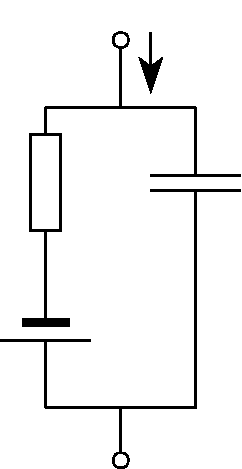
\includegraphics[scale=.5]{figures/LIF.pdf}};
  \node[anchor=south] at (1.2,3.8) {presynaptic activation};
  \node[anchor=south] at (1.8,3.1) {$I(t)$};
  \node[anchor=south] at (-.3,2.2) {$R$};
  \node[anchor=south] at (1,2.2) {$C$};
  \node[anchor=south] at (-.5,1) {$u_\mathrm{rest}$};
  \draw [decorate,decoration={brace,amplitude=5pt}]
(2.5,3.1) -- (2.5,.5) node [anchor=west,black,midway,xshift=1em] {$u(t)$};
\end{tikzpicture}
\caption[Electrical circuit of a leaky integrate and fire neuron]{Electrical circuit of a leaky integrate and fire neuron. The unit saves incoming charges $I(t)$ called the presynaptic activation into the capacitor $C$, essentially summing them up or \emph{integrating} them. Once the charge reaches a threshold value, the neuron discharges or \emph{fires} (postsynaptic activation). The dissipation of ions through the cell's membrane is modelled by allowing the charge to \emph{leak} through the resistor $R$.}\label{fig:LIF}
\end{figure}\noindent
As the impulses are extremely sparse in time, LIF neurons generally allow for much more efficient computation compared to the neurons found in CNNs. Alternatively this can be thought of as higher information density: the frequency of rate-based codes corresponds to averaging a temporal window and therefore a loss of information over the pulse-based code. While it is possible to use a code based on the firing rate, the full potential of spiking neurons is only levelled, when information is also encoded in the timing of the firing \cite{bohte2002unsupervised,bohte2004evidence,hopfield1995pattern}. A single spiking neuron, encoding information in the rate and temporal patterns of its spike train, can replace hundreds of second generation neurons\footnote{The first generation of neurons or neural networks generally refers to networks consisting of linear neurons (called \emph{perceptrons}), while the second generation is understood to refer to architectures using artificial neurons with nonlinear activation functions, such as CNNs as discussed in section \ref{section:cnn}. Networks based on the dynamics of spiking neurons are known as third generation neural networks.} \cite{gerstner2002spiking,maass1997networks,rieke1999spikes}. The synapses interconnecting the spiking neurons in a SNN are scaled by learnable weights, the same as CNNs. Many of the ideas developed for CNNs, like perceptive fields, different types of layers, batch normalization etc., can be directly applied to SNNs. There are however two major differences: (i) the input data must be encoded into spike trains and (ii) the synaptic weights must be learned based on the dynamics of the spiking neurons. In computer vision experiments it is quite common to use rate based stochastic encoding schemes. The spike trains are generated by sampling from a stochastic distribution (e.g. Poisson) with firing rates proportional to the intensity of the pixels \cite{diehl2015unsupervised}. SNNs may be trained using biologically plausible algorithms. Learning rules which strengthen synapses based on the timing of spikes are referred to as \emph{Hebbian} learning and often colloquially summarized by the phrase \enquote{Cells that fire together, wire together} \cite{hebbs1949organization}. Mathematically, the change in synaptic weight $\Delta w_{ij}$ between two neurons $i$ and $j$ may be expressed as
\begin{align}
    \Delta w_{ij} \propto v_i v_j.
\end{align}
with $v_i$ the activity of neuron $i$. Because there is no labelled data or any training signal involved, Hebbian learning rules are inherently unsupervised. Methods that consider the precise timing and order of pre- and postsynaptic spikes are known as \emph{spike-timing-dependent plasticity} (STDP). In STDP the firing of a postsynaptic spike increases the strength of presynaptic weights that fired shortly before. This is referred to as \emph{long term potentiation} (LTP). The reverse order leads to a decrease in synaptic strength and is conversely known as \emph{long term depression} (LTD). The change in weight $\Delta w_i$ for a synapse from a presynaptic neuron $i$ according to STDP can also be expressed mathematically.
\begin{align}
    \Delta w_i = \sum_{f=1}^N\sum_{n=1}^NF\qty(t_n^{(j)}-t_f^{(i)})
\end{align}
Where $t_n^{(j)}$ and $t_f^{(i)}$ denote the times of the firing of spikes by the postsynaptic neuron $j$ and the presynaptic neuron $i$ respectively. The STDP function $F$ or \emph{learning window} largely determines the specific behavior of the STDP model. A popular choice, that also corresponds well with experimental findings \cite{song2000competitive} is given by
\begin{align}
    F(\Delta t) = \begin{cases}
      A_+\exp(-\frac{\Delta t}{\tau_+})\qq{for} \Delta t < 0\\
      -A_-\exp(-\frac{\Delta t}{\tau_-})\qq{for} \Delta t \geq 0.
    \end{cases}
\end{align}
With $A_{+/-}$ linear coefficients and $\tau_{+/-}$ a kind of decay defining the size of the window.
\begin{figure}
    \centering
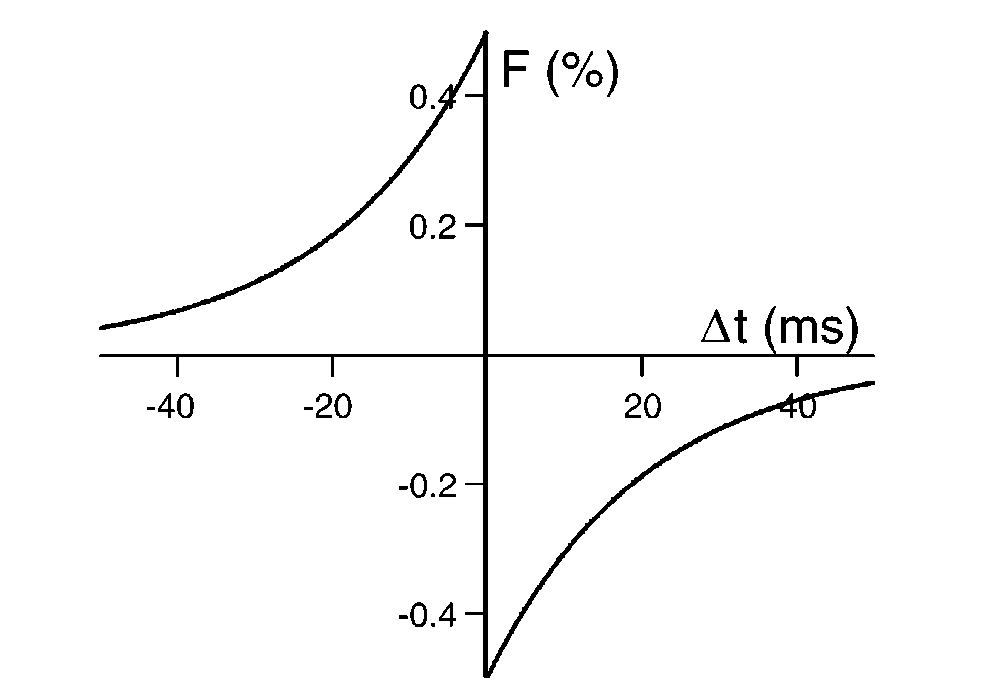
\includegraphics[]{figures/stdp-window.png}
\caption[STDP window function]{STDP window function from \cite{song2000competitive}. The change in conductance for a synapse due to a single pre- and postsynaptic spike pair in STDP is proportional to $F(\Delta t)$ with $\Delta t$ the time of the presynaptic spike minus the time of the postsynaptic spike. In this figure, $F$ was expressed as a percentage.}\label{fig:stdp}
\end{figure}\noindent
While research into biologically plausible learning algorithms is ongoing \cite{bing2018survey,bartunov2018assessing}, they are generally outperformed by engineering methods such as gradient descent\footnote{Gradient descent is generally regarded as not a realistic option for how the brain learns. This is because it requires a teaching signal in the form of labelled data and calculates a gradient specific to each neuron based on that signal.} in tasks that allow for supervised training (e.g. classification and regression) \cite{diehl2015unsupervised}. Training a deep network of spiking neurons discriminatively using gradient descent with backpropagation is difficult, because the LIF neuron's activity is non-differentiable at the time of spikes (cf. figure \ref{fig:spiketrain}). For the supervised training of feed-forward\footnote{Feed-forward networks allow propagation of signals in only one direction and do not contain any cycles. While there are other successful architectures like recurrent neural networks (RNNs), restricted Boltzmann machines (RBMs) or deep belief networks (DBNs), they do not play an important role in computer vision tasks compared to CNNs.} networks using backpropagation, there are generally two established approaches. The first trains a second generation network and afterwards converts it to a SNN for inference. The second type of method directly optimizes an objective function using an approximation of spatio-temporal gradient descent similar to backpropagation in CNNs. Recently, deep spiking convolutional networks have been trained successfully usinig backpropagation by treating the discontinuities at spike times as noise i.e. approximating a smooth signal \cite{10.3389/fnins.2016.00508, panda2016unsupervised}. While all approaches to SNNs currently do not perform quite as well as CNNs on computer vision tasks, they are inherently computationally less expensive and could at the very least lead to power efficient hardware implementation in the form of neuromorphic systems\footnote{A neuromorphic system is a hardware implementation of neural circuitry in silico that allows for fast and direct computation on neural networks.} \cite{hopkins2018spiking}.
\begin{figure}
    \centering
\def\svgwidth{\textwidth}
\import{figures/}{spiketrain.pdf_tex}
\caption[Presynaptic spike train, membrane potential and postsynaptic spike train of a LIF neuron]{Presynaptic spike train, membrane potential and postsynaptic spike train of a LIF neuron. The three plots are synchronous in time. A presynaptic spike adds a charge to the membrane potential that decays over time. Once the membrane potential reaches the threshold $\vartheta$, the neuron discharges, generating a postsynaptic spike and resetting to resting potential $u_\mathrm{rest}$. Note the discontinuity whenever a pre- or postsynaptic neuron fires.}\label{fig:spiketrain}
\end{figure}\noindent
\section{Limitations of Artificial Neural Networks}

Convolutional layers in CNNs use translated replicas (via weight sharing) of learned feature detectors. The rational behind this is that knowledge about good features in one part of the image may be useful in other regions as well. While this has proved quite a powerful semantic and grants CNNs a measure of invariance to translations, they do not generalize well to other transformations. This requires the networks to be trained using a large number of training images, covering all desired variations in viewpoint, scale, lighting, color etc. It is common to artificially extend the training set by applying image transformations. This process is known as \emph{data augmentation}.  \cite{wong2016understanding,perez2017effectiveness}. Nevertheless the process of creating datasets for (deep) neural networks is quite time consuming and expensive. Even if labelled data is available, training is computationally expensive and can take several days \cite{Lee:2016:HVC:3012029.3012067,silver2016mastering}. The same can be said for inference on trained networks, which often requires great computational resources and still suffers from relatively high latency \cite{dong2009high}. These drawbacks along with the fact that high computational costs come with large energy requirements, make real time and especially mobile applications under constrained resources difficult. Another shortcoming of CNNs is due to their use of pooling layers. The bottle-neck architecture of CNNs allows them to use a growing number of feature maps with large receptive fields, representing high-level features and shapes. With every pooling operation however, information on the location of features is lost. This means that CNNs cannot learn the precise spatial relations between a whole and its parts. For tasks like facial recognition however, part-whole relations play an important role \cite{tanaka2016parts}. 

SNNs on the other hand try to avoid the limitations imposed by the high computational costs and energy requirements of CNNs by mimicking the sparse encoding of information in spikes as observed in brains. SNNs running on neuromorphic hardware are extremely energy efficient and are able to operate in real time by design, independent of the size and topology of the network. Still, the computation on current neuromorphic circuity is only a qualitative approximation of digitally simulated spiking neurons and even those do currently not approach state of the art CNN accuracy in computer vision tasks \cite{indiveri2011neuromorphic,diehl2015unsupervised}. Biological systems, especially the visual cortex of the primate brain, are not subject to these limitations \cite{stone2018rotation,isbister2018new}. It therefore stands to reason that all of these challenges can be met and that findings from biology and neuroscience may hold a clue as to how to engineer solutions.

Recently an ANN architecture consisting of groups of neurons called \emph{capsules} has been proposed as a possibly biologically plausible alternative for CNNs in computer vision systems. Capsule networks can be thought of as a visual attention mechanism, that encodes poses between features. Additionally, the activation functions and pooling operations found in CNNs are replaced by a sophisticated routing organism, that retains positional information. In theory this grants capsule networks a measure of viewpoint invariance as well as access to precise part-whole relations throughout the network. As capsule networks are still rate-coded and trained by supervised SGD with backpropagation, they fall somewhere inbetween CNNs and SNNs in regards to biological plausibility, but are possibly more expressive than CNNs. The theory behind capsules is explored in detail in the next chapter.